%!TEX root = ../../../main.tex

\chapter[Coupling NDs]{Coupling \Nds to Photonic Structures}	\label{ch::coupling}

	In the last chapter, we saw that the spectroscopic properties of \sivs vary strongly among individual \nds.
	\Nds are further implemented in photonic structures for the application in metrology as well as in quantum cryptography or quantum computing.
	Therefore, it is important to have a good knowledge of the spectroscopic properties of the individual \todo{think of other word} \siv.
	A preselection of \nds including an \siv with optimal properties is performed.
	These properties contain both spectroscopic parameters as well as technical parameters for the \pp process.
	Spectroscopic parameters contain narrow linewidth, high countrates and single photon emission, the technical parameters include a size of the \nds hosting the \siv bigger than \SI{70}{nm} and how isolated they lie on the substrate surface.
	The selected \nd is then transferred to a target structure.
	In the scope of this thesis, \nds including \sivs were coupled to two different kinds of structures:
	\begin{itemize}
		\item \Vcsels: The aim is to create a hybrid-integrated \sps, where an electric current is employed to create single photons. The diamond containing an \siv is placed directly on the beam output. Hence the \siv is directly pumped by the laser beam. This system is interesting for metrological applications, as it is the major building block for a portable device ready to calibrate single photon detectors.
		\item Plasmonic Nanoantennas: The aim is to enhance \pl intensity. As described in previous chapters, not only \ZPL position and \lw, but also the \pl intensity varies strongly among individual \sivs. However, in metrology a photon flux rate high enough to be measured by a low optical flux detector is needed \cite{Vaigu2017}. This increase in intensity is achieved by coupling the \sivs in \nds to plasmonic antennas.
	\end{itemize}


	\section{Additional Experimental Methods} \label{sec::methods_coupling}


	To couple \nds to photonic structures, we pursued several different methods: 
	\begin{enumerate} 
		\item Directly spin-coat the structures with a \nd solution and consecutively look for a structure containing a \nds with an \siv exhibiting the desired spectroscopic properties. This method was tried with the antenna structures, as there are many antenna structures on one substrate (see \Cref{subfig::antenna_structures_sem}), therefore there is a chance that a suited \nd is incidentally ends up at the right spot. However, it is not suitable for the VCSELs, first because of the morphology of the VCSELs and secondly, because there is a very limited number of VCSELs on one substrate.
		\item \label{item::pp}Use an \ir substrate covered with \nds containing \sivs, look for a suited \nd and transfer it with a \pp technique using a nanomanipulator. The nanomanipulator is essentially a thin tip in a \sem. The \ir substrate is prepeocessed with markers, to record the position of the preselected \nd. The huge advantage is that the very best suited \nd can be preselected. However, disadvantages of this process include the electron radiation during the \pp process, which might affect \siv \fl and the further restriction that the \nds must be big enough to be picked up with the nanomanipulator. 
		\item Similar to method \ref{item::pp}, however the transfer is performed with an \afm. While this method has the advantage that the \nds are not irradiated with electrons, the disavantage is that it is not possible to  observe the picking process in real time. The area of the preselected \nd has to be scanned after every pick-up try, which is very time consuming and therefore was not further pursued after some trials.
	\end{enumerate}

	In the following paragraphs, the \pp technique of method \ref{item::pp} is described in more detail.
	It is the coupling method most extensivly deployed in the scope of this thesis and requires a range of experimental setups. 
	The \pp process was carried out with major help from \pauly.
	The nanomanipulator setup was provided by the same group.
	\\
	\subsection{Nanomanipulator} \label{subsec::nanomanipulator}
	% -Nanomanipulator
	% 	Probleme mit Spitze
	% \begin{figure}[tp]		
	% 	\centering
	% 	\testbox{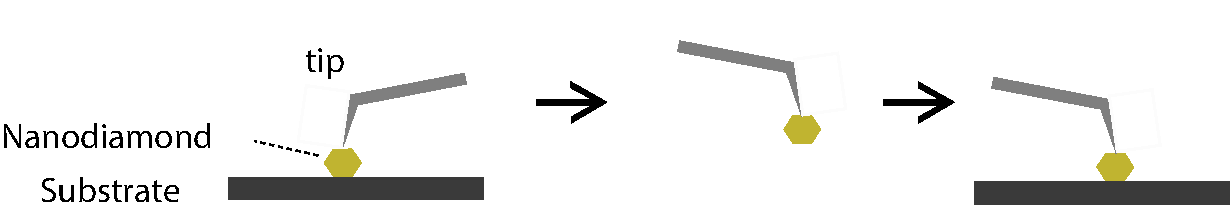
\includegraphics[trim = 0 0 0 0,  clip= true, width = 0.3\textwidth]{./pics/pp_sketch.pdf}}
	% 	\caption{Sketch of the \pp process exploiting a nanomanipulator.}
	% 	\label{fig::pp_sketch}
	% \end{figure}

	\begin{figure}[tp]
		\begin{subfigure}[t]{ 0.49\linewidth}
			\centering
			\testbox{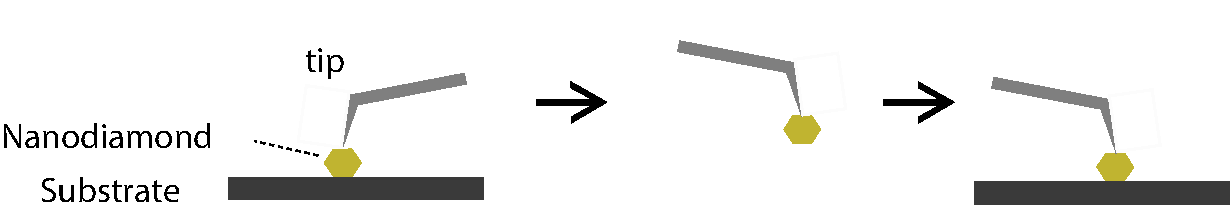
\includegraphics[trim = 0 0 0 0,  clip= true, width = \textwidth]{./pics/pp_sketch.pdf}}
			\caption{}
			\label{subfig::pp_sketch}
		\end{subfigure}
		\hfill
		\begin{subfigure}[t]{ 0.49\linewidth}
			\centering
			\testbox{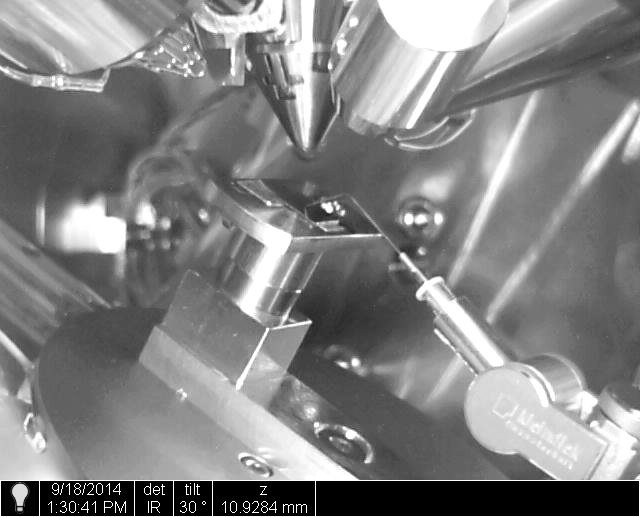
\includegraphics[trim = 0 0 0 0,  clip= true, width = \textwidth]{./pics/nanomanipulator_image_arrows.png}}
			\caption{}
			\label{subfig::nanomanipulator_image}
		\end{subfigure}
		\caption{(a) Sketch of the \pp process exploiting a nanomanipulator. (b) Image of the nanomanipulator mounted in the FIB. The arrows indicate the degrees of freedom of motion of the nanomanipulator. The custom made workbench is situated in the middle of the picture. On top of it, there is a \SI{1}{\centi\meter\squared} substrate with coated \nds, the nanomanipulator tip pointing to the middle of it. Behind it, there is the target \vcsel. Perpendicular to the workbench, the objective of the electron microscope can be seen. The pointier cone perpendicular to the image top image edge is the objective of the \fib.}
	\end{figure}

	In general, nanomanipulator is a tip mounted inside an SEM, allowing manipulation and visualization of the manipulation process at the same time.
	The one used for our experiments was built by the company Kleindiek (model MM3A-EM) and has a changeable tungsten tip (see \cref{subfig::nanomanipulator_image}).
	It is mouted inside a Thermo Scientific\texttrademark{} Helios NanoLab\texttrademark{}  DualBeam\texttrademark{} microscope, which combines a \fib and an electron microscope.
	The bent nanomanipulator tip has 3 degrees of freedom: up/down and left/right both in an arc up to \SI{240}{\degree} and \SI{12}{\milli\metre} in/out (see arrows in \cref{subfig::nanomanipulator_image}). 
	Before nanomanipulation the tip was "sharpened" with the focussed ion beam by etching away  tungsten with gallium ions.
	This sharpening was performed to meet the size criteria necessary to pick up the \nds.
	In \cref{subfig::nanomanipulator_tip} the sharpened tip is shown (the radius of curvature amounts to \SI{100}{\nano\meter}).
	The small tip sticking out of the bigger cone is the sharp tip used for \pp.


	\subsection{Determination of The Position of \Nds} \label{subsec::position}

	\begin{figure}[tp]
		\begin{subfigure}[t]{ 0.49\linewidth}
			\centering
			\testbox{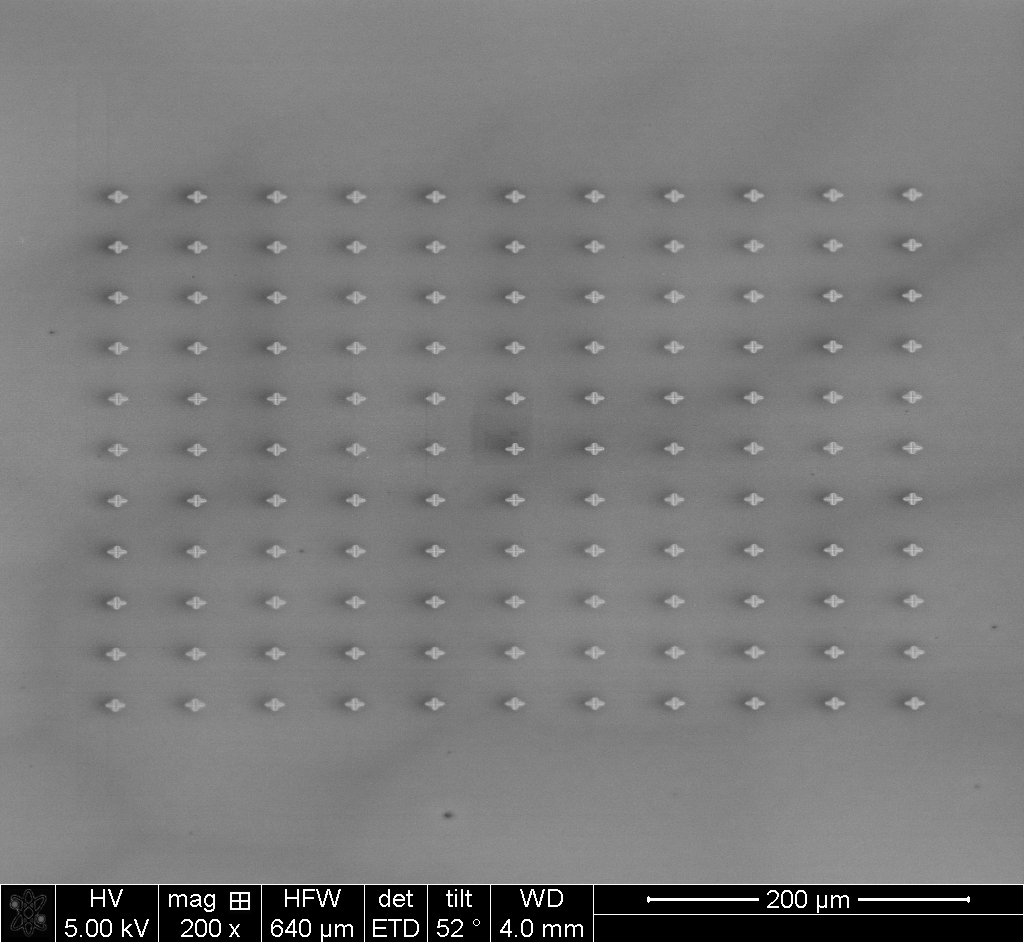
\includegraphics[trim = 0 0 0 0,  clip= true, width = \textwidth]{./pics/M09-13_mitte_131209_01.png}}
			\caption{}
			\label{subfig::cross_markers}
		\end{subfigure}
		\hfill
		\begin{subfigure}[t]{ 0.49\linewidth}
			\centering
			\testbox{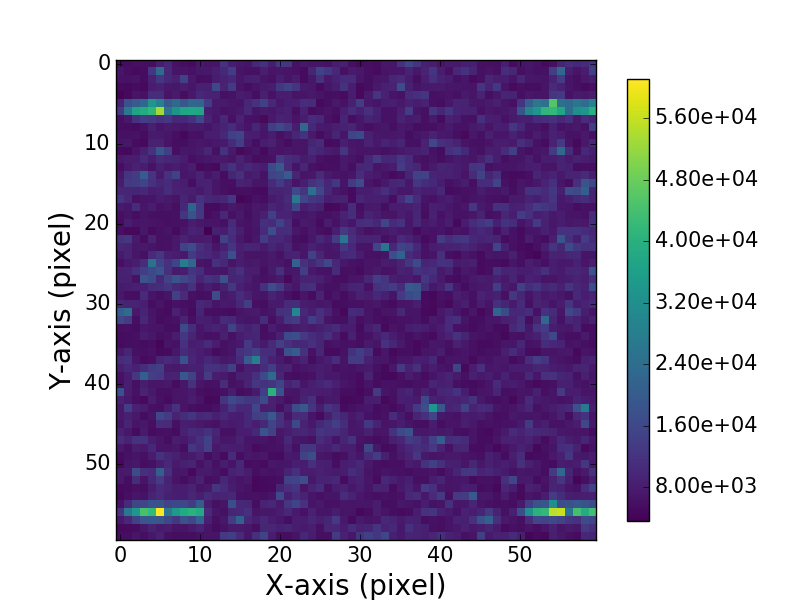
\includegraphics[trim = 0 0 0 0,  clip= true, width = \textwidth]{./pics/114-02_2APD.png}}
			\caption{}
			\label{subfig::cross_marker_whitelightscan}
		\end{subfigure}
		\caption{(a) Overview of a field of cross markers. The field spans \num{0.5}\ensuremath{\times}\SI{0.5}{\milli\meter} (b) White light scan of an area with a cross marker in all four corners.}
		\label{fig::<fig>}
	\end{figure}

	An \nd pre-characterized in the confocal setup exhibiting the preferred spectroscopic properties has to be found again in the SEM setup where the nanomanipulator is installed.
	Therefore, we milled cross markers into the \ir coating of the \si substrate using the \fib prior to spin-coating the substrate with \nd solution.\todo{fib parameter}
	The crosses' size is \num{10}$\times$\SI{10}{\micro\meter\squared} are exhibit a nominal depth of \SI{40}{nm}.
	Four crosses are the cornerpoints of a \num{50}$\times$\SI{50}{\micro\meter\squared} sqaure.
	The \num{10}$\times$\num{10} crosses spaned one field of crosses; we usually put 3 fields of crosses on one substrate.
	\\
	To record the position of a \nd \wrt a cross marker, we used two different methods:
	\begin{itemize}
		\item Scanning the sample in the confocal setup while a white light source illuminates the sample from the side in an acute angle. The edges of the cross markers are visible in the fluorescence scan. After turning the white light lamp off, the same area is scanned once more to record the fluorescence from the \sivs. An overlay of the two images identifies the position of fluorescent \sivs \wrt the cross markers.\todo{put in a pic of whitelightscan} The disadvantage of this method is, that it takes a lot of time, as every scan has to be performed twice. Also, as only \fl scans are performed, no information of the \nds is accessible. Such information comprises of the size of the individual \nds and whether the \nds lie isolated on the substrate surface. These parameters are only available during the \pp process in the SEM. An emitter with optimal optical properties can turn out not to be suited for \pp just before the process itself, hence the time spent to optically characterize an emitter was in vain.
		\item A more efficient method is scanning the substrate first in a commercial \lsm \todo{specs}. The \lsm is a confocal microscope where the focus of a laser is used to obtain the height of a structure. \todo{verify info}It is possible to scan a whole field of cross markers in several minutes. The obtained image is a greyscale image, where the greyscale corresponds to the height deviation of a structure. Therefore, both the crosses and the \nds appear in darker shades of grey. So in contrast to the previous method, information on the size and isolation of the \nds is accessible. After scanning the substrate with the \lsm, it is put into the confocal setup. While observing the surface with the CCD camera (\cref{fig::place_ccd}), a specific cross marker is chosen as the starting point of a \fl scan. Comparing the \lsm image and a \fl scan, fluorescent dots of the \fl scan are attributed to \nds in the \lsm scan (see \cref{subfig::cross_laser_scan,subfig::pp_pl_scan}).
	\end{itemize}

	\subsection{The \PP Process}

	\begin{figure}[tp]
		\begin{subfigure}[t]{ 0.49\linewidth}
			\centering
			\testbox{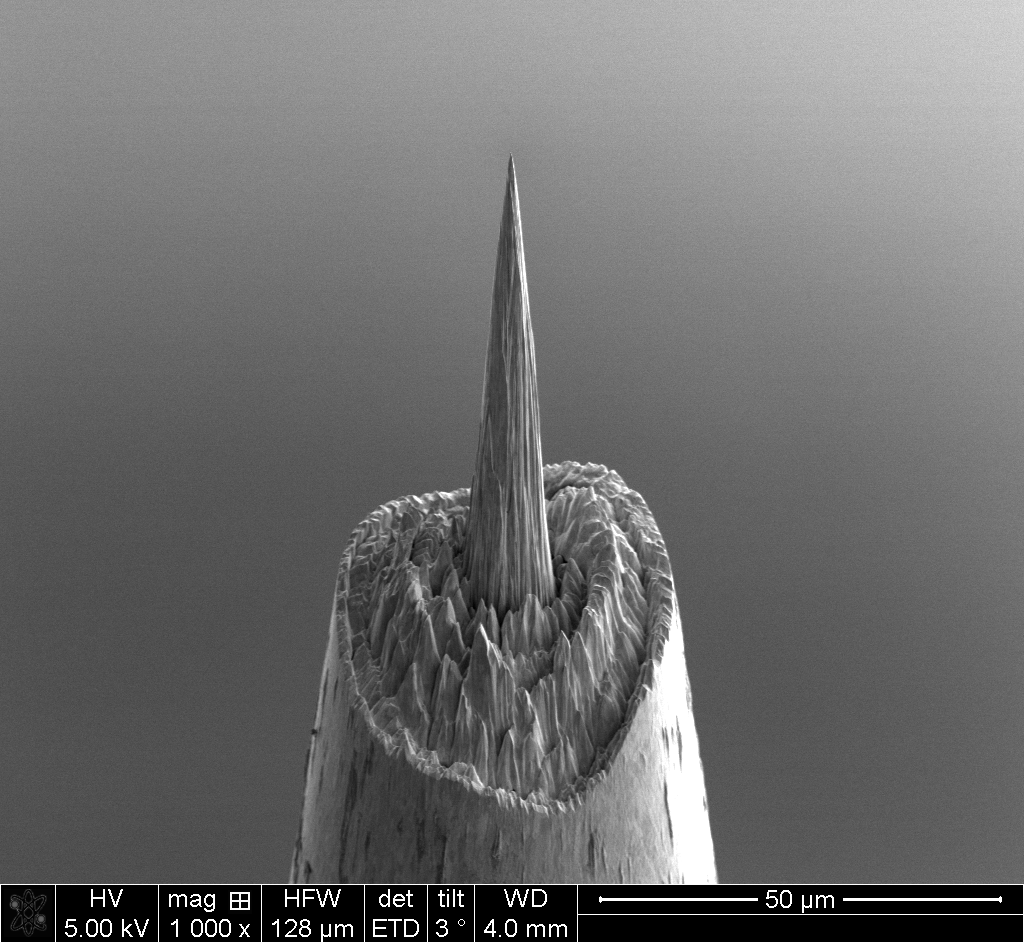
\includegraphics[trim = 0 0 0 0,  clip= true, width = \textwidth]{./pics/Tip2_140826_03.png}}
			\caption{}
			\label{subfig::nanomanipulator_tip}
		\end{subfigure}
		\hfill
		\begin{subfigure}[t]{ 0.49\linewidth}
			\centering
			\testbox{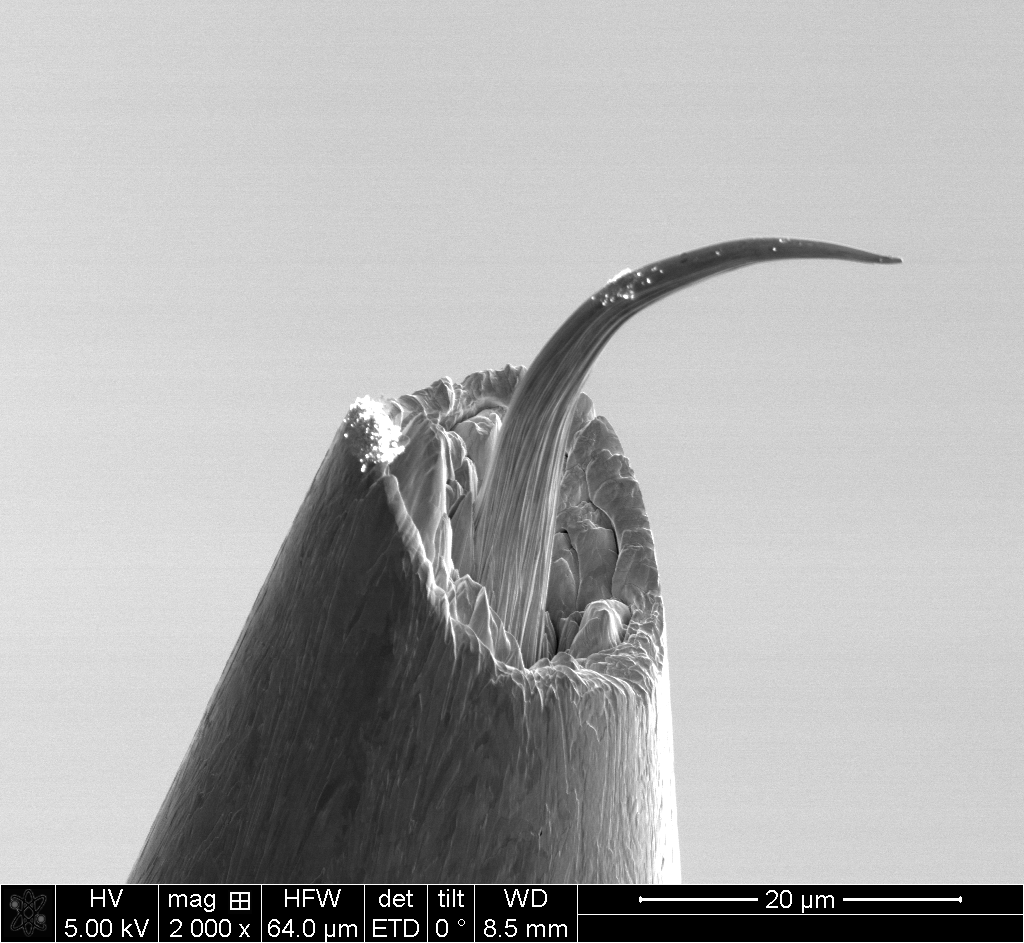
\includegraphics[trim = 0 0 0 0,  clip= true, width = \textwidth]{./pics/M05-13_140826_05.png}}
			\caption{}
			\label{subfig::nanomanipulator_tip_bent}
		\end{subfigure}
		\caption{}
	\end{figure}

	After we identified \nds as well-suited for transfer to the target structure, both the substrate with the \nds and the target structure were mounted inside the SEM. 
	The process was performed using a high resolution mode with a low acceleration voltage of the SEM of \SI{1}{\kilo\electronvolt} and a current of \SI{1.7}{\nano\ampere}.
	The tip is approached to the pre-selected \nd from above.
	As the SEM objective is mounted above the \np, the proximity the \np tip  to the \nd is not observable.
	The proximity is indirectly estimated by the shadow the tip casts onto the substrate and the focus.
	The first method is used for the coarse approachment of the tip to the \nd: The closer the tip gets to the \nd, the closer the shadow of the tip coincides with the \nd position.
	Exploiting the focus as an estimate for the proximity of the tip is used for fine adjustment during the last stage of the approachment.
	This is done as follows: 
	At the end of the coarse movement, the tip of the \np is still some distance above the \nd.
	The SEM is focused on the \nd, therefore the \np tip is out of focus and appears blurry.
	As the tip is approached, it moves further and further into focus, its image becoming sharper, until the it touches the \nd.
	As this is a tricky process, sometimes the tip was approached with too much force and was destroyed in the process (\cref{subfig::nanomanipulator_tip_bent}).
	\\
	When performed correctly, due to adhesion, the \nd sticks to the \np tip when the both get in contact (\cref{subfig::pick_antenna_sem}).
	The nanomanipulator is then moved to the target structure and the same approachment procedure is applied.
	Dependent on the material of the target structure, the \nd either sticks to the structure right away due to higher adhesion forces between the \nd and the structure (as is the case for the golden plasmonic antennas).
	Or the \nd has to be "wiped off" of the \np tip in a sideways motion.
	In either way it is possible to place the \nd within a precision of a few nanometers.
	\\
	% The used SEM has a special high resolution mode. 
	% With this mode it is possible, to obtain high resolution images at a low acceleration voltage.
	% The pitfall is that for this mode a small working distance of \SI{5}{mm} is necessary. 
	% This working distance is too small for to use the nanomanipulator at the same time.
	% Therefore, first we identified the position of the pre-selected \nd in high resolution mode in the SEM, marked its position in the iamge, switched to normal working mode and 
	% - Hochaufloesungsmodus geringer arbeitsabstand von 5mm, higher magn. field
	% - Abloesen von Diamanten (BASD + CVD) von Substrat im Ultraschallbad kann dazu fuehren, dass Substrat mitabgeloest wird) -> in Kalilauge aufloesen LII, S96
	% - warum nicht einfach neue CVD-Diamanten herstellen, wie die, die am Anfang meiner Diss so gut funktioniert haben -> Dichte am Substrat zu hoch zum Aufpicken



